%%%%%%%%%%%%%%%%%%%%%%%%%%%%%%%%%%%%%%%%%%%%%%%%%%%%%%%%%%%%%%%%%%%%%%%%%%%%%%%%%%
\begin{frame}[fragile]\frametitle{}
\begin{center}
{\Large Introduction to Deep Learning}
\end{center}
\end{frame}


%%%%%%%%%%%%%%%%%%%%%%%%%%%%%%%%%%%%%%%%%%%%%%%%%%%%%%%%%%%%%%%%%%%%%%%%%%%%%%%%%%
\begin{frame}[fragile]\frametitle{Deep Learning is}
\begin{itemize}
\item A big bang of Artificial Intelligence.
\item making Spark of innovation of most amazing break-through
\item having Super human capabilities in image recognition
\item making remarkable progress in text, speech, automobiles
\item beating humans at Chess and Go
\end{itemize}
\begin{center}
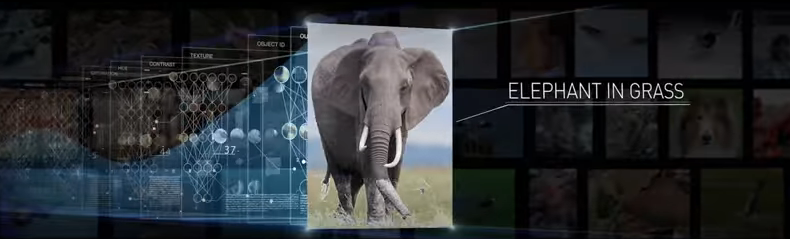
\includegraphics[width=\linewidth,keepaspectratio]{dl26}
\end{center}
{\tiny (The Deep Learning Revolution - Nvidia)}
\end{frame}

%%%%%%%%%%%%%%%%%%%%%%%%%%%%%%%%%%%%%%%%%%%%%%%%%%%%%%%%%%%%%%%%%%%%%%%%%%%%%%%%%%
\begin{frame}[fragile]\frametitle{History}
\begin{center}
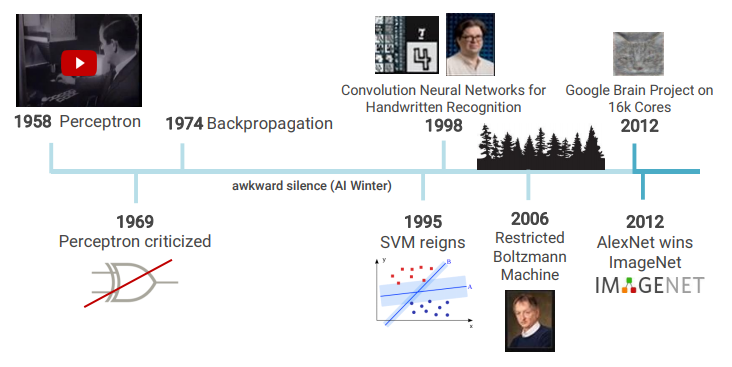
\includegraphics[width=\linewidth,keepaspectratio]{ai37}
\end{center}
{\tiny (Deep Learning - The Past, Present and Future of Artificial Intelligence - Lukas Masuch)}
\end{frame}


%%%%%%%%%%%%%%%%%%%%%%%%%%%%%%%%%%%%%%%%%%%%%%%%%%%%%%%%%%%%%%%%%%%%%%%%%%%%%%%%%%
\begin{frame}[fragile]\frametitle{Interest : Google Trends}
\begin{center}
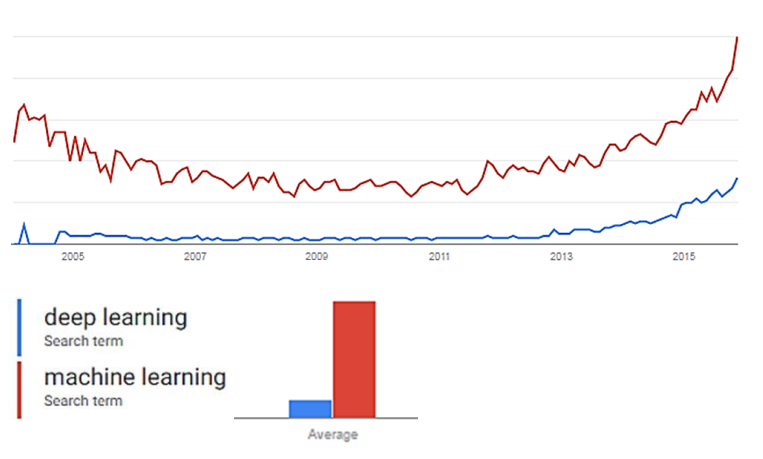
\includegraphics[width=\linewidth,keepaspectratio]{dl27}
\end{center}
{\tiny (Deep Learning - The Past, Present and Future of Artificial Intelligence - Lukas Masuch)}
\end{frame}

%%%%%%%%%%%%%%%%%%%%%%%%%%%%%%%%%%%%%%%%%%%%%%%%%%%%%%%%%%%%%%%%%%%%%%%%%%%%%%%%%%
\begin{frame}[fragile]\frametitle{Academic Publications in Deep Learning}
\begin{center}
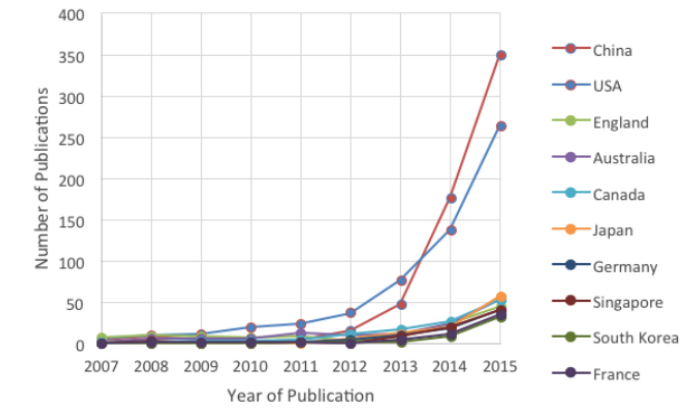
\includegraphics[width=\linewidth,keepaspectratio]{dl28}
\end{center}
{\tiny (Deep Learning - The Past, Present and Future of Artificial Intelligence - Lukas Masuch)}
\end{frame}
%%%%%%%%%%%%%%%%%%%%%%%%%%%%%%%%%%%%%%%%%%%%%%%%%%%
\begin{frame}[fragile] \frametitle{Why Deep Learning is taking off?}
Deep learning is taking off due to a large amount of data available through the digitization of the society, 
faster computation and innovation in the development of neural network algorithm. 

\begin{center}
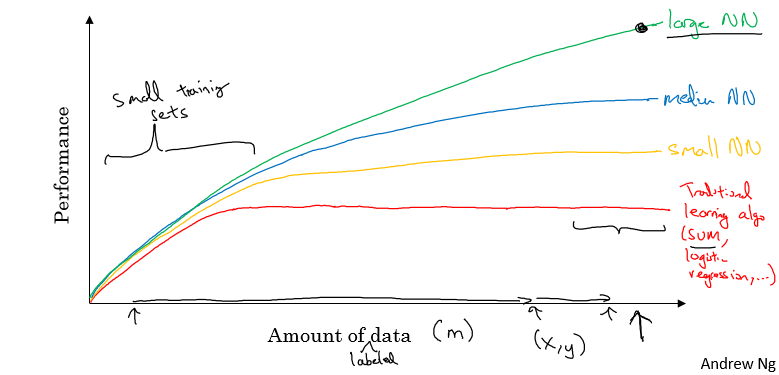
\includegraphics[width=\linewidth,keepaspectratio]{ai19}
\end{center}


\tiny{(Reference: Introduction to Neural Networks - Andrew Ng)}

\end{frame}

%%%%%%%%%%%%%%%%%%%%%%%%%%%%%%%%%%%%%%%%%%%%%%%%%%%%%%%%%%%%%%%%%%%%%%%%%%%%%%%%%%
\begin{frame}[fragile]\frametitle{What changed?}
Old wine in new bottles
\begin{center}
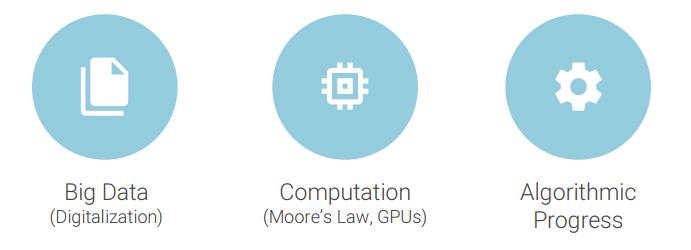
\includegraphics[width=\linewidth,keepaspectratio]{ai40}
\end{center}
{\tiny (Deep Learning - The Past, Present and Future of Artificial Intelligence - Lukas Masuch)}
\end{frame}



%%%%%%%%%%%%%%%%%%%%%%%%%%%%%%%%%%%%%%%%%%%%%%%%%%%%%%%%%%%%%%%%%%%%%%%%%%%%%%%%%%
\begin{frame}[fragile]\frametitle{Deep Learning: Hype or Reality}
\begin{center}
\includegraphics[width=\linewidth,keepaspectratio]{dl29}
\end{center}
{\tiny (Deep Learning - The Past, Present and Future of Artificial Intelligence - Lukas Masuch)}
\end{frame}


%%%%%%%%%%%%%%%%%%%%%%%%%%%%%%%%%%%%%%%%%%%%%%%%%%%
\begin{frame}[fragile] \frametitle{AI ML DL: What's the difference?}

\begin{itemize}
\item Artificial Intelligence: mimicking human intelligence
\item Machine Learning: Automating Learning with features. 
\item There could be programmed (hand coded) AI, that's not Machine Learning
\item Machine Learning could be for non AI activities, like automation
\item Deep Learning: Neural network with no input features
\end{itemize}
\end{frame}

%%%%%%%%%%%%%%%%%%%%%%%%%%%%%%%%%%%%%%%%%%%%%%%%%%%%%%%%%%
\begin{frame}[fragile] \frametitle{AI ML DL: What's the difference?}
\begin{center}
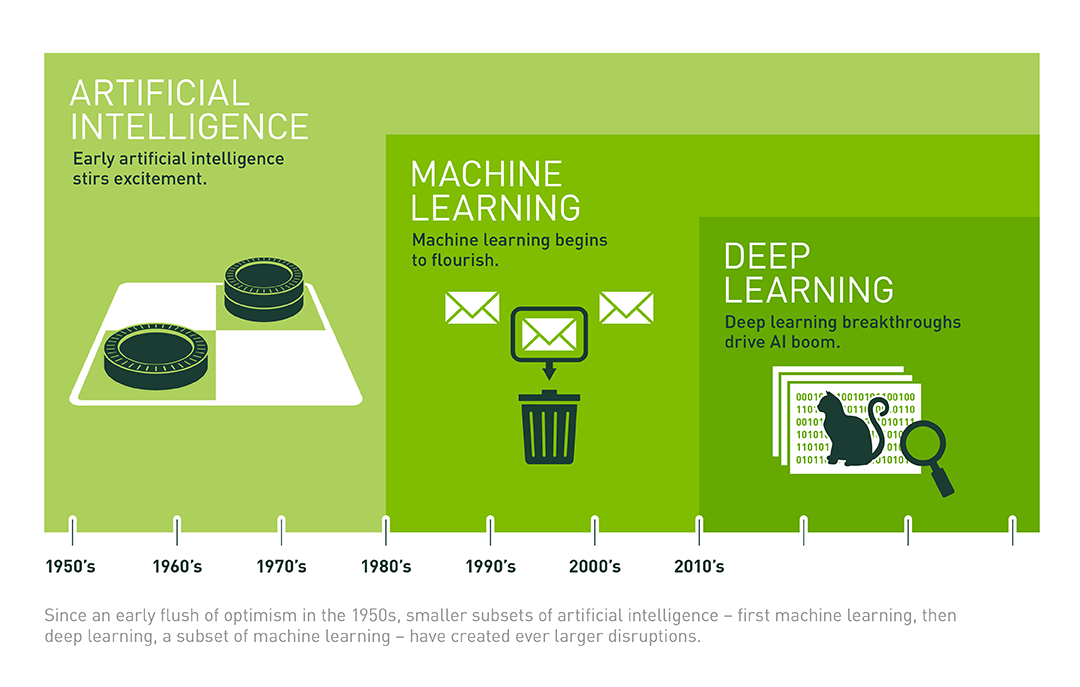
\includegraphics[width=\linewidth,keepaspectratio]{aimldl}
\end{center}
\tiny{(Reference: The Difference Between AI, Machine Learning, and Deep Learning - NVIDIA Blog)}
\end{frame}

%%%%%%%%%%%%%%%%%%%%%%%%%%%%%%%%%%%%%%%%%%%%%%%%%%%%%%%%%%
\begin{frame}[fragile] \frametitle{Types of AI}
\begin{center}
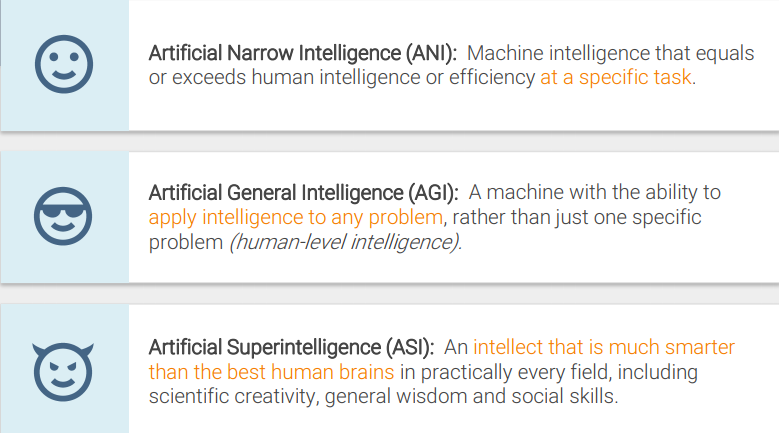
\includegraphics[width=\linewidth,keepaspectratio]{ai28}
\end{center}
{\tiny (Deep Learning - The Past, Present and Future of Artificial Intelligence - Lukas Masuch)}
\end{frame}

%%%%%%%%%%%%%%%%%%%%%%%%%%%%%%%%%%%%%%%%%%%%%%%%%%%%%%%%%%
\begin{frame}[fragile] \frametitle{State of AI}
\begin{center}
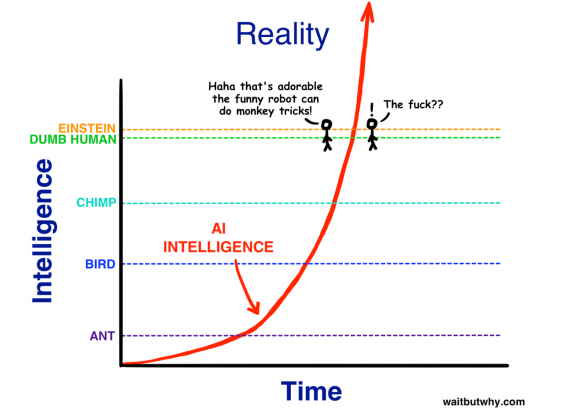
\includegraphics[width=0.8\linewidth,keepaspectratio]{ai29}
\end{center}
{\tiny (Deep Learning - The Past, Present and Future of Artificial Intelligence - Lukas Masuch)}
\end{frame}


%%%%%%%%%%%%%%%%%%%%%%%%%%%%%%%%%%%%%%%%%%%%%%%%%%%
\begin{frame}[fragile] \frametitle{Paradigms of Software Development}

\begin{itemize}
\item Rule based
\item Machine Learning
\item Deep Learning

\end{itemize}

\end{frame}


%%%%%%%%%%%%%%%%%%%%%%%%%%%%%%%%%%%%%%%%%%%%%%%%%%%
\begin{frame}[fragile] \frametitle{Rule based : Digit recognition}
\begin{center}
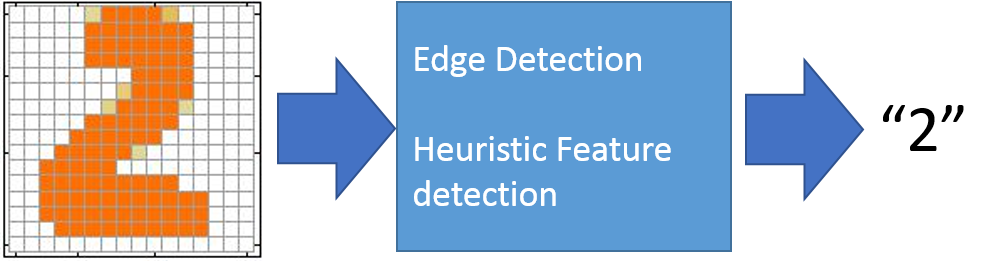
\includegraphics[width=\linewidth,keepaspectratio]{rulebaseddigits}
\end{center}

{\tiny (Image Credit: Deep Learning Tutorial - Hung yi Lee)}


\end{frame}

%%%%%%%%%%%%%%%%%%%%%%%%%%%%%%%%%%%%%%%%%%%%%%%%%%%
\begin{frame}[fragile] \frametitle{Machine Learning : Digit recognition}
\begin{center}
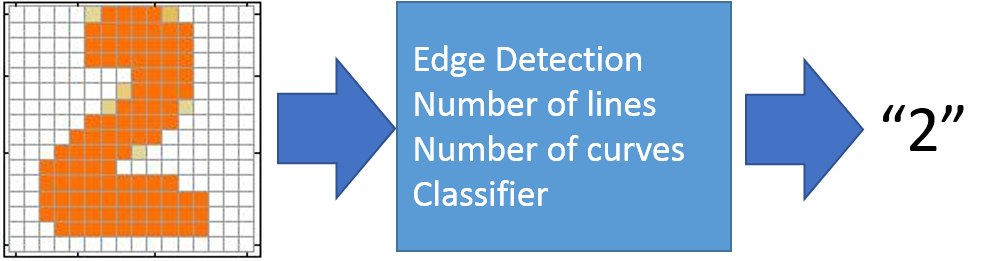
\includegraphics[width=\linewidth,keepaspectratio]{machinelearningdigits}
\end{center}
{\tiny (Image Credit: Deep Learning Tutorial - Hung yi Lee)}
\end{frame}

%%%%%%%%%%%%%%%%%%%%%%%%%%%%%%%%%%%%%%%%%%%%%%%%%%%
\begin{frame}[fragile] \frametitle{Deep Learning : Digit recognition}
\begin{center}
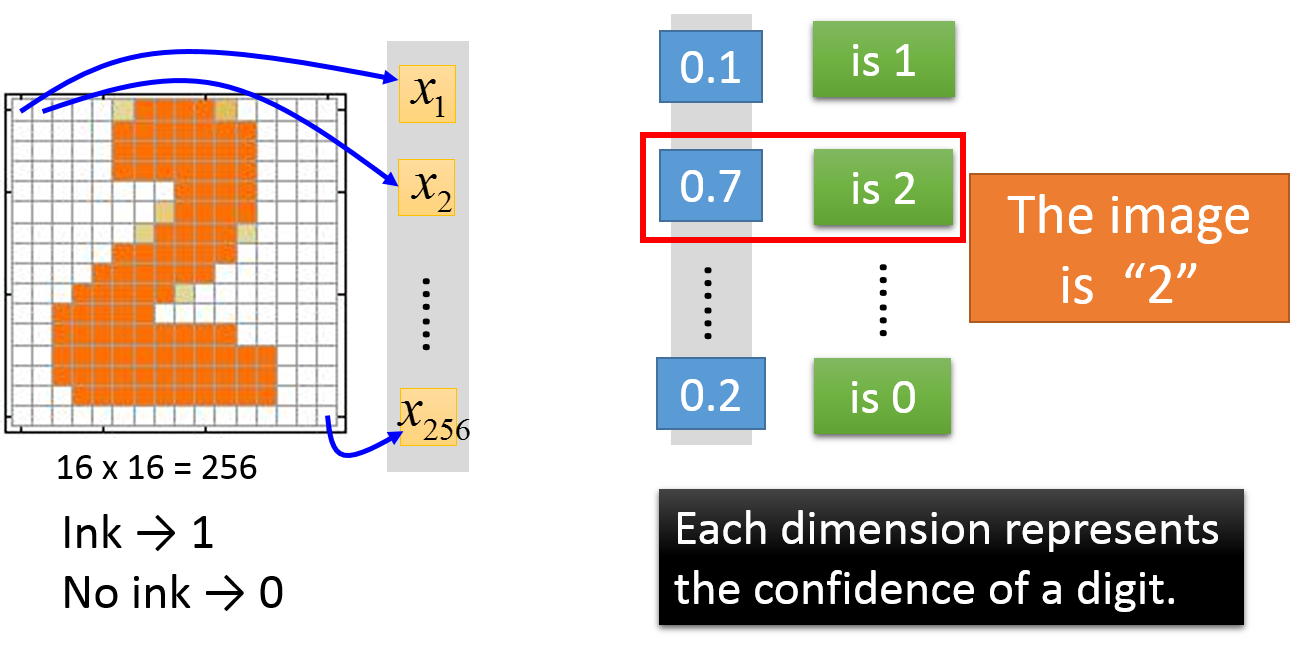
\includegraphics[width=0.8\linewidth,keepaspectratio]{deeplearningdigits}
\end{center}

\end{frame}

%%%%%%%%%%%%%%%%%%%%%%%%%%%%%%%%%%%%%%%%%%%%%%%%%%%%%%%%%%
\begin{frame}[fragile]\frametitle{Machine Learning Deep Learning}
\begin{center}
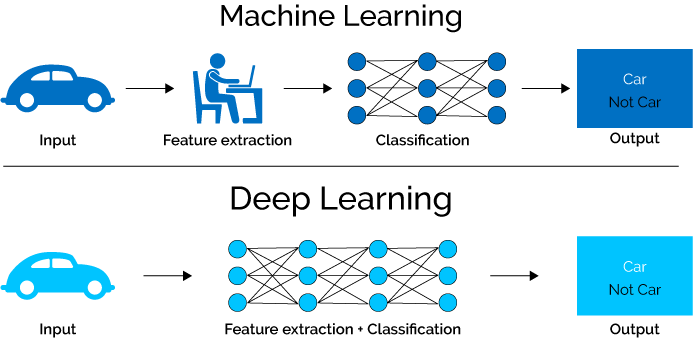
\includegraphics[width=\linewidth,keepaspectratio]{mldl1}
\end{center}
\tiny{(Reference: https://medium.com/@xenonstack/log-analytics-with-deep-learning-and-machine-learning-20a1891ff70e)}
\end{frame}

%%%%%%%%%%%%%%%%%%%%%%%%%%%%%%%%%%%%%%%%%%%%%%%%%%%%%%%%%%
\begin{frame}[fragile] \frametitle{Machine Learning}
\begin{center}
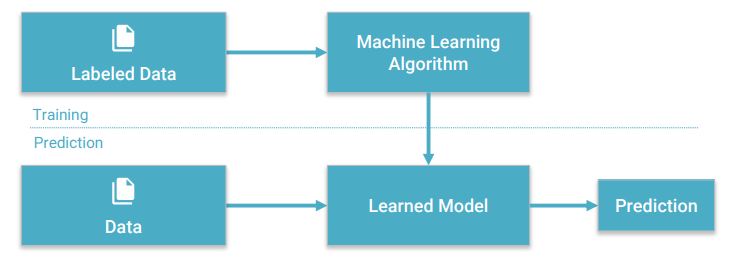
\includegraphics[width=\linewidth,keepaspectratio]{ai30}
\end{center}
Provides various techniques that can learn from and make predictions on data
{\tiny (Deep Learning - The Past, Present and Future of Artificial Intelligence - Lukas Masuch)}
\end{frame}

%%%%%%%%%%%%%%%%%%%%%%%%%%%%%%%%%%%%%%%%%%%%%%%%%%%%%%%%%%
\begin{frame}[fragile] \frametitle{Machine Learning}
\begin{center}
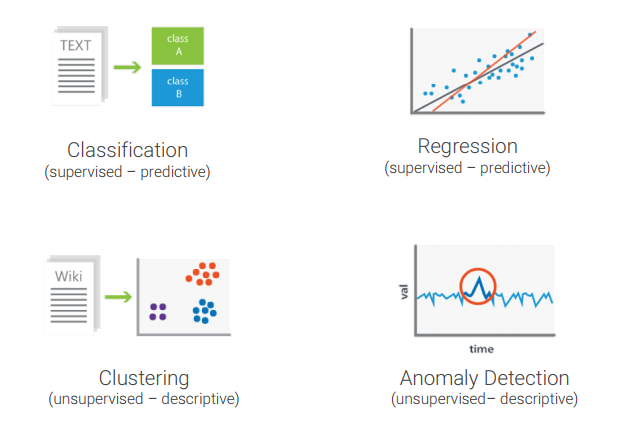
\includegraphics[width=\linewidth,keepaspectratio]{ai31}
\end{center}
{\tiny (Deep Learning - The Past, Present and Future of Artificial Intelligence - Lukas Masuch)}
\end{frame}

%%%%%%%%%%%%%%%%%%%%%%%%%%%%%%%%%%%%%%%%%%%%%%%%%%%%%%%%%%
\begin{frame}[fragile] \frametitle{Deep Learning}
\begin{center}
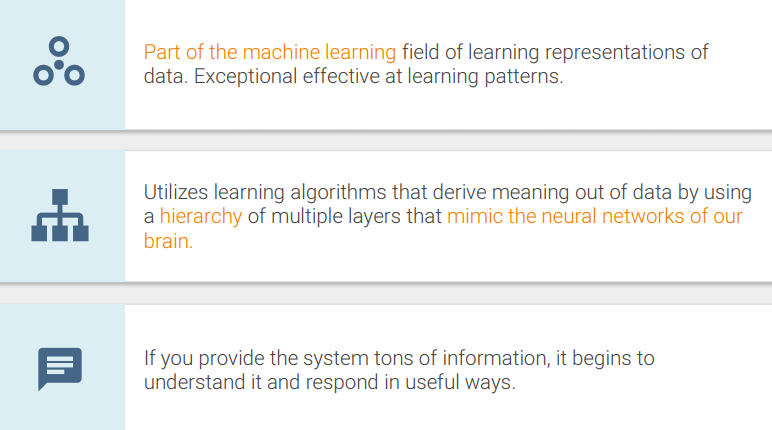
\includegraphics[width=\linewidth,keepaspectratio]{ai32}
\end{center}
{\tiny (Deep Learning - The Past, Present and Future of Artificial Intelligence - Lukas Masuch)}
\end{frame}


%%%%%%%%%%%%%%%%%%%%%%%%%%%%%%%%%%%%%%%%%%%%%%%%%%%%%%%%%%
\begin{frame}[fragile] \frametitle{Deep Learning}
\begin{center}
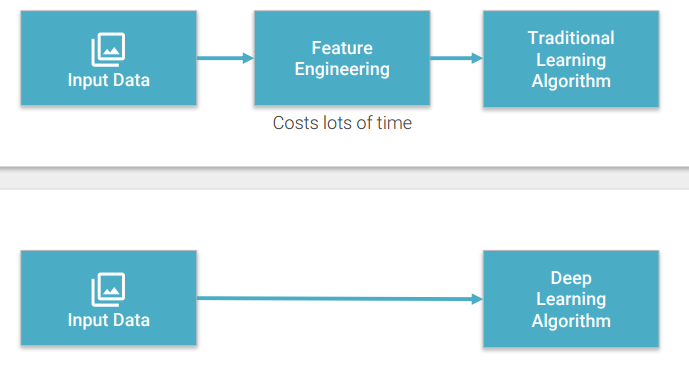
\includegraphics[width=\linewidth,keepaspectratio]{ai36}
\end{center}
{\tiny (Deep Learning - The Past, Present and Future of Artificial Intelligence - Lukas Masuch)}
\end{frame}

%%%%%%%%%%%%%%%%%%%%%%%%%%%%%%%%%%%%%%%%%%%%%%%%%%%%
%\begin{frame}[fragile] \frametitle{Deep Learning : Digit recognition}
%\begin{center}
%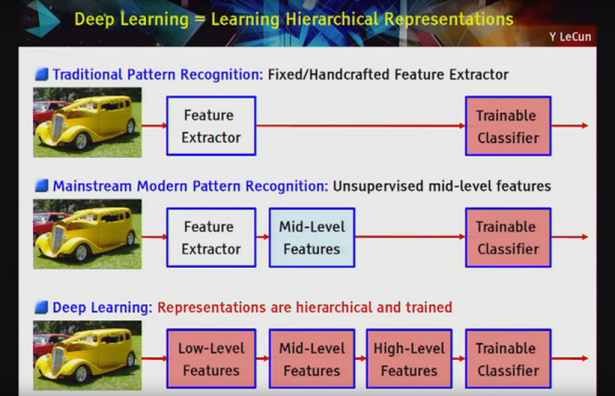
\includegraphics[width=0.8\linewidth,keepaspectratio]{mldl}
%\end{center}
%\end{frame}

%%%%%%%%%%%%%%%%%%%%%%%%%%%%%%%%%%%%%%%%%%%%%%%%%%%
\begin{frame}[fragile] \frametitle{Deep Learning == Neural Nets }

\begin{itemize}
\item Main idea of deep learning: transform the input space into outputs via higher level abstractions.
\item Neural Net architectures are made up of perceptrons (similar to neurons) 
\item Each neuron carries certain transformations on inputs coming to it.
\item Collection of such neurons with various types of transformations, can create desired overall transformation.
\end{itemize}
\end{frame}



%%%%%%%%%%%%%%%%%%%%%%%%%%%%%%%%%%%%%%%%%%%%%%%%%%%
\begin{frame}[fragile] \frametitle{Inspiration}

\begin{itemize}
\item Attempts to simulate biological neural systems
\item  Animal brains have complex learning systems consisting of closely interconnected sets of neurons
\item  Human brain contains approximately 1011 neurons
\item  Each connected on average to 10,000 other neurons
\item  Total of 1,000,000,000,000,000 = 1015 connections
\end{itemize}

\begin{center}
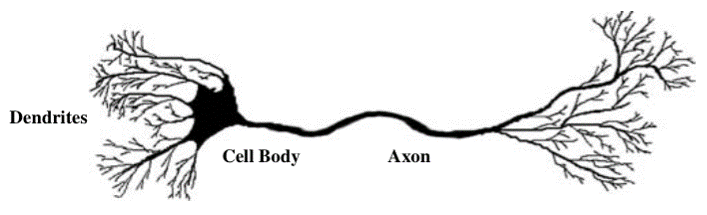
\includegraphics[width=0.8\linewidth,keepaspectratio]{brain_neuron}
\end{center}

\end{frame}

%%%%%%%%%%%%%%%%%%%%%%%%%%%%%%%%%%%%%%%%%%%%%%%%%%%%%%%%%%%%%%%%%%%%%%%%%%%%%%%%%%
\begin{frame}[fragile] \frametitle{Inspiration}
An artificial neuron contains a nonlinear activation function and has several
incoming and outgoing weighted connections. 
\begin{center}
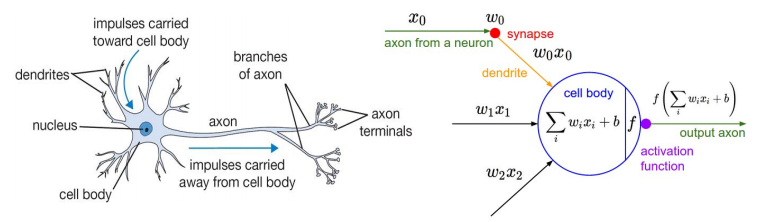
\includegraphics[width=\linewidth,keepaspectratio]{ai43}
\end{center}
{\tiny (Deep Learning - The Past, Present and Future of Artificial Intelligence - Lukas Masuch)}
\end{frame}


%%%%%%%%%%%%%%%%%%%%%%%%%%%%%%%%%%%%%%%%%%%%%%%%%%%%%%%%%%
\begin{frame}[fragile] \frametitle{Inspiration}
\begin{center}
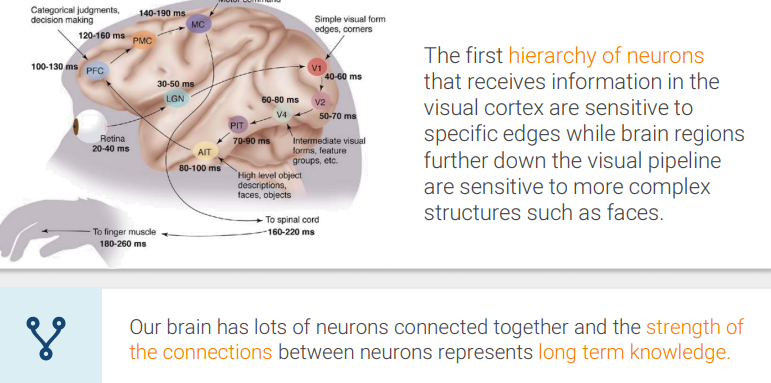
\includegraphics[width=\linewidth,keepaspectratio]{ai33}
\end{center}
{\tiny (Deep Learning - The Past, Present and Future of Artificial Intelligence - Lukas Masuch)}
\end{frame}

%%%%%%%%%%%%%%%%%%%%%%%%%%%%%%%%%%%%%%%%%%%%%%%%%%%%%%%%%%
\begin{frame}[fragile] \frametitle{Inspiration}
\begin{itemize}
\item A deep neural network consists of a hierarchy of layers, whereby each layer
transforms the input data into more abstract representations (e.g. edge to
nose to face). 
\item The output layer combines those features to make predictions.
\end{itemize}
\begin{center}
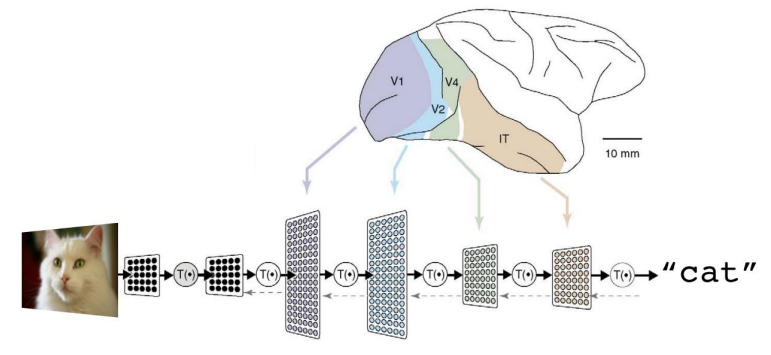
\includegraphics[width=0.6\linewidth,keepaspectratio]{ai34}
\end{center}
{\tiny (Deep Learning - The Past, Present and Future of Artificial Intelligence - Lukas Masuch)}
\end{frame}

%%%%%%%%%%%%%%%%%%%%%%%%%%%%%%%%%%%%%%%%%%%%%%%%%%%%%%%%%%
\begin{frame}[fragile] \frametitle{Inspiration}
\begin{center}
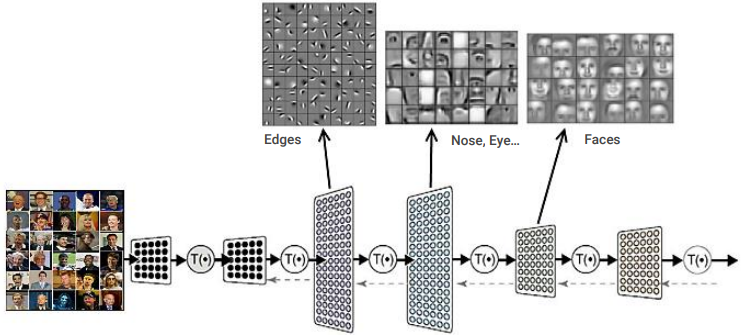
\includegraphics[width=\linewidth,keepaspectratio]{ai35}
\end{center}
{\tiny (Deep Learning - The Past, Present and Future of Artificial Intelligence - Lukas Masuch)}
\end{frame}
%%%%%%%%%%%%%%%%%%%%%%%%%%%%%%%%%%%%%%%%%%%%%%%%%%%
\begin{frame}[fragile] \frametitle{Inspiration}

\begin{center}
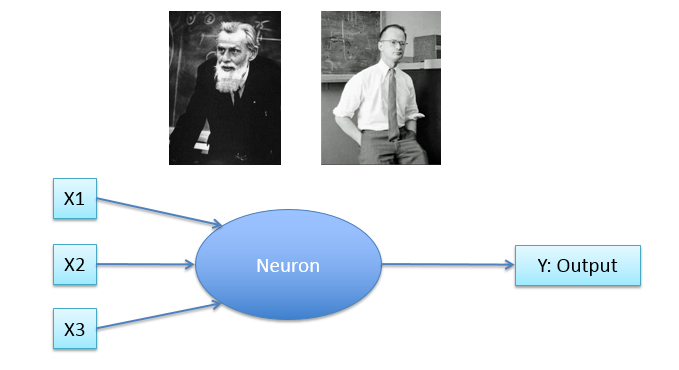
\includegraphics[width=0.8\linewidth,keepaspectratio]{ai7}
\end{center}
\tiny{(Reference: Warren McCulloch and Walter Pitts (1943) ``A Logical Calculus of the Ideas Immanent in Nervous Activity''. )}
\end{frame}

%%%%%%%%%%%%%%%%%%%%%%%%%%%%%%%%%%%%%%%%%%%%%%%%%%%
\begin{frame}[fragile] \frametitle{Inspiration}

\begin{center}
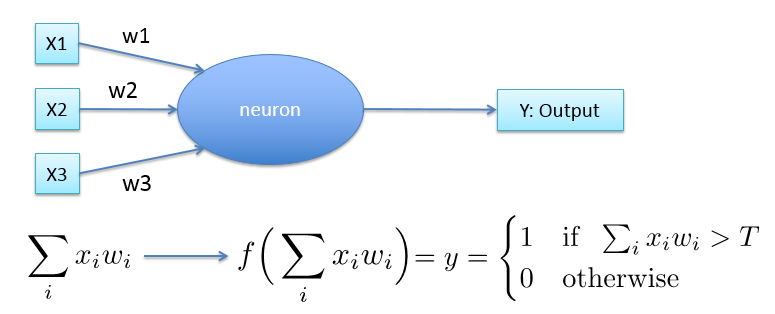
\includegraphics[width=0.8\linewidth,keepaspectratio]{ai8}
\end{center}
\tiny{(Reference:The perceptron model (Rosenblatt, 1957) )}
\end{frame}



%
%%%%%%%%%%%%%%%%%%%%%%%%%%%%%%%%%%%%%%%%%%%%%%%%%%%%
%\begin{frame}[fragile] \frametitle{Paradigms of Software Development}
%
%\begin{itemize}
%\item Rule based
%\item Machine Learning
%\item Deep Learning
%
%\end{itemize}
%
%\end{frame}
%
%
%%%%%%%%%%%%%%%%%%%%%%%%%%%%%%%%%%%%%%%%%%%%%%%%%%%%
%\begin{frame}[fragile] \frametitle{Rule based : Digit recognition}
%\begin{center}
%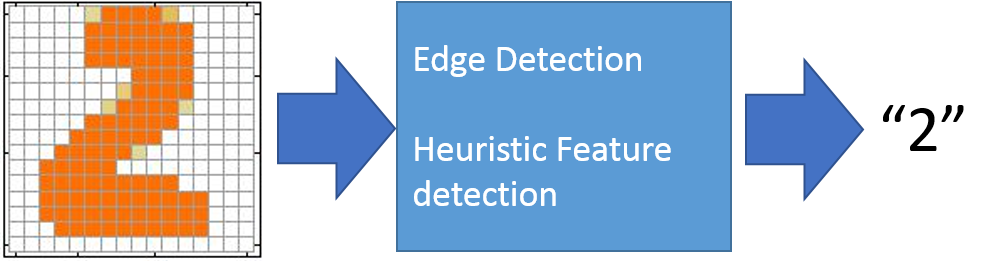
\includegraphics[width=\linewidth,keepaspectratio]{rulebaseddigits}
%\end{center}
%
%{\tiny (Image Credit: Deep Learning Tutorial - Hung yi Lee)}
%
%
%\end{frame}
%
%%%%%%%%%%%%%%%%%%%%%%%%%%%%%%%%%%%%%%%%%%%%%%%%%%%%
%\begin{frame}[fragile] \frametitle{Machine Learning : Digit recognition}
%\begin{center}
%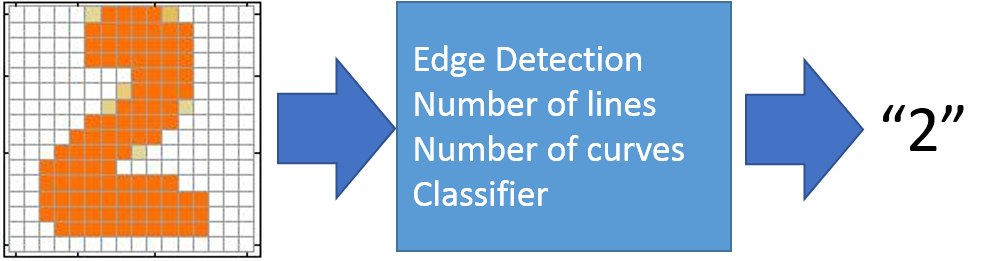
\includegraphics[width=\linewidth,keepaspectratio]{machinelearningdigits}
%\end{center}
%{\tiny (Image Credit: Deep Learning Tutorial - Hung yi Lee)}
%\end{frame}
%
%%%%%%%%%%%%%%%%%%%%%%%%%%%%%%%%%%%%%%%%%%%%%%%%%%%%
%\begin{frame}[fragile] \frametitle{Deep Learning : Digit recognition}
%\begin{center}
%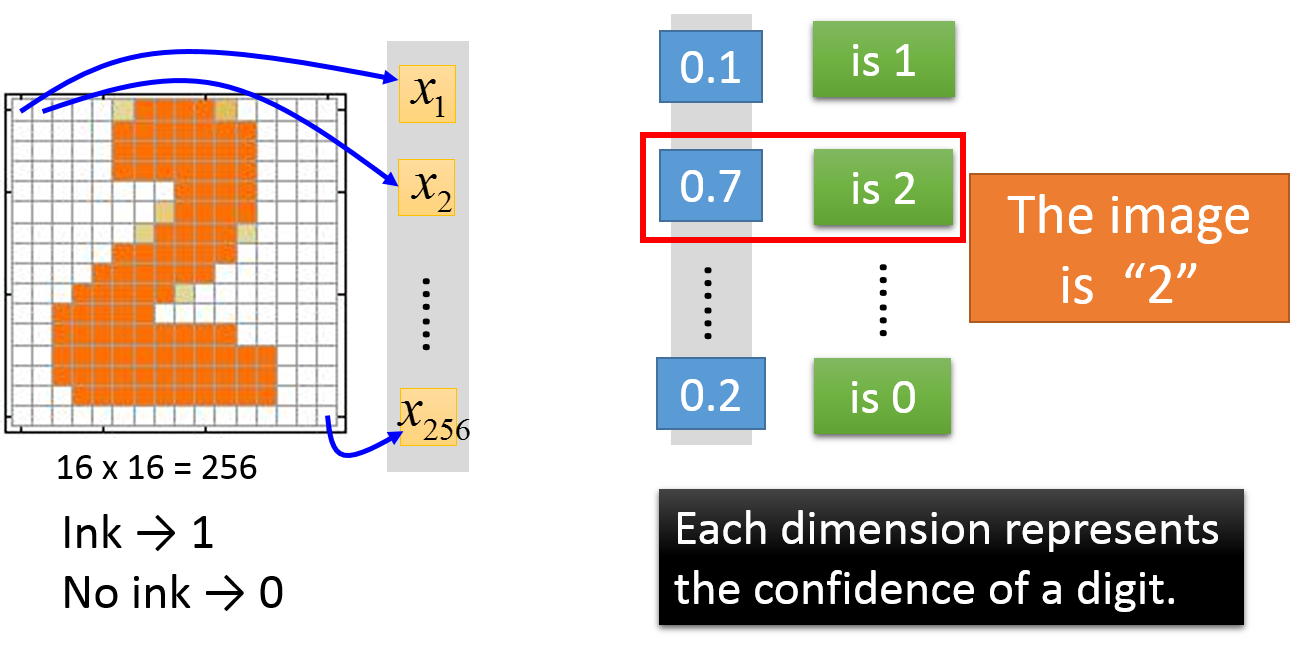
\includegraphics[width=0.8\linewidth,keepaspectratio]{deeplearningdigits}
%\end{center}
%
%\end{frame}
%
%%%%%%%%%%%%%%%%%%%%%%%%%%%%%%%%%%%%%%%%%%%%%%%%%%%%%%%%%%%
%\begin{frame}[fragile]\frametitle{Machine Learning Deep Learning}
%\begin{center}
%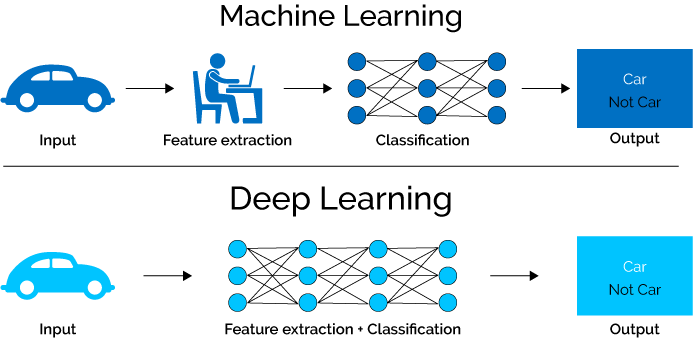
\includegraphics[width=\linewidth,keepaspectratio]{mldl1}
%\end{center}
%\tiny{(Reference: https://medium.com/@xenonstack/log-analytics-with-deep-learning-and-machine-learning-20a1891ff70e)}
%\end{frame}
%
%
%%%%%%%%%%%%%%%%%%%%%%%%%%%%%%%%%%%%%%%%%%%%%%%%%%%%%
%%\begin{frame}[fragile] \frametitle{Deep Learning : Digit recognition}
%%\begin{center}
%%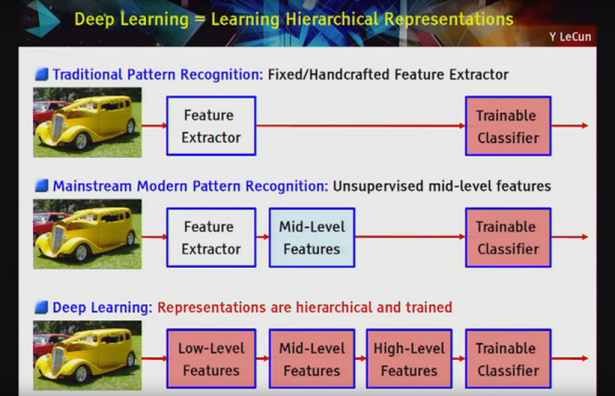
\includegraphics[width=0.8\linewidth,keepaspectratio]{mldl}
%%\end{center}
%%\end{frame}
%
%%%%%%%%%%%%%%%%%%%%%%%%%%%%%%%%%%%%%%%%%%%%%%%%%%%%
%\begin{frame}[fragile] \frametitle{Deep Learning == Neural Nets }
%
%\begin{itemize}
%\item Main idea of deep learning: transform the input space into outputs via higher level abstractions.
%\item Neural Net architectures are made up of perceptrons (similar to neurons) 
%\item Each neuron carries certain transformations on inputs coming to it.
%\item Collection of such neurons with various types of transformations, can create desired overall transformation.
%\end{itemize}
%\end{frame}
%
%
%
%%%%%%%%%%%%%%%%%%%%%%%%%%%%%%%%%%%%%%%%%%%%%%%%%%%%
%\begin{frame}[fragile] \frametitle{Inspiration}
%
%\begin{itemize}
%\item Attempts to simulate biological neural systems
%\item  Animal brains have complex learning systems consisting of closely interconnected sets of neurons
%\item  Human brain contains approximately 1011 neurons
%\item  Each connected on average to 10,000 other neurons
%\item  Total of 1,000,000,000,000,000 = 1015 connections
%\end{itemize}
%
%\begin{center}
%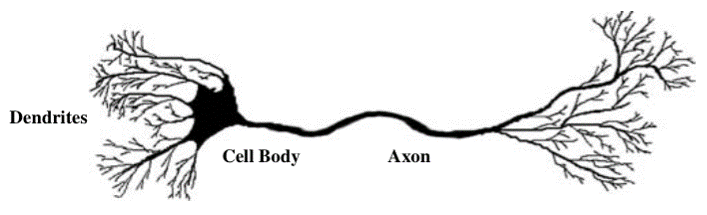
\includegraphics[width=0.8\linewidth,keepaspectratio]{brain_neuron}
%\end{center}
%
%\end{frame}
%
%%%%%%%%%%%%%%%%%%%%%%%%%%%%%%%%%%%%%%%%%%%%%%%%%%%%
%\begin{frame}[fragile] \frametitle{Inspiration}
%
%\begin{center}
%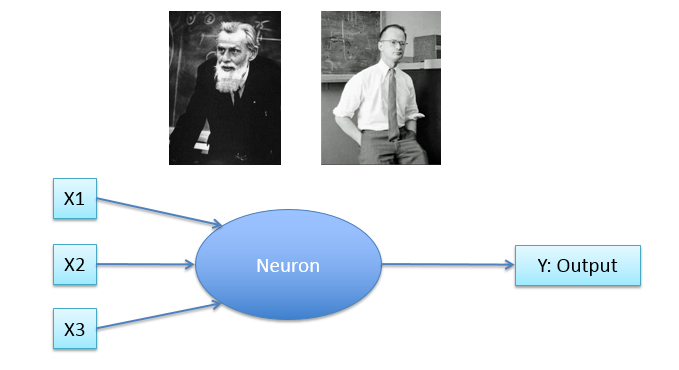
\includegraphics[width=0.8\linewidth,keepaspectratio]{ai7}
%\end{center}
%\tiny{(Reference: Warren McCulloch and Walter Pitts (1943) ``A Logical Calculus of the Ideas Immanent in Nervous Activity''. )}
%\end{frame}
%
%%%%%%%%%%%%%%%%%%%%%%%%%%%%%%%%%%%%%%%%%%%%%%%%%%%%
%\begin{frame}[fragile] \frametitle{Inspiration}
%
%\begin{center}
%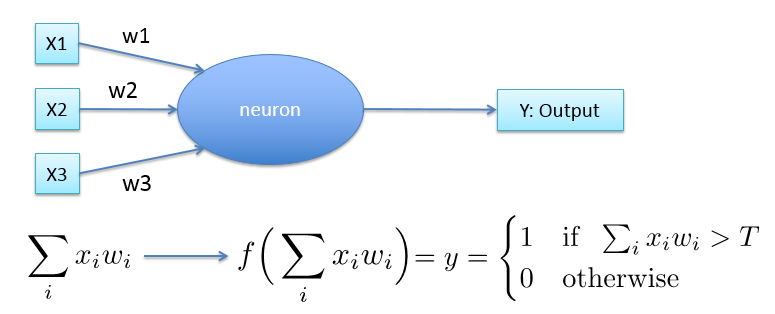
\includegraphics[width=0.8\linewidth,keepaspectratio]{ai8}
%\end{center}
%\tiny{(Reference:The perceptron model (Rosenblatt, 1957) )}
%\end{frame}
%
%%%%%%%%%%%%%%%%%%%%%%%%%%%%%%%%%%%%%%%%%%%%%%%%%%%%
%\begin{frame}[fragile] \frametitle{How does it work?}
%Intuition: Consider a black box that takes numerical inputs, does something
%to them, and gives a numerical output. 
%
%\begin{center}
%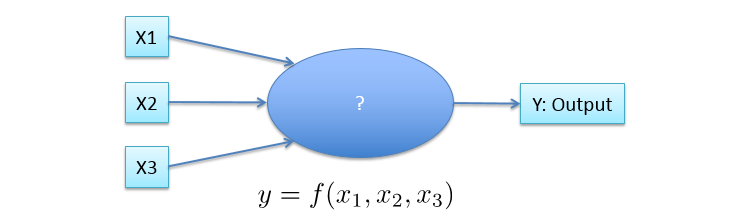
\includegraphics[width=0.8\linewidth,keepaspectratio]{ai9}
%\end{center}
%Wouldn't it be great to know the generic relationship between inputs and outputs? 
%\tiny{(Reference: Neural Networks - Dr. Long Tran-Thanh)}
%\end{frame}

%%%%%%%%%%%%%%%%%%%%%%%%%%%%%%%%%%%%%%%%%%%%%%%%%%%
\begin{frame}[fragile] \frametitle{Sum of the inputs}
Idea 1: what if we consider f as a sum of the inputs? 
\begin{center}
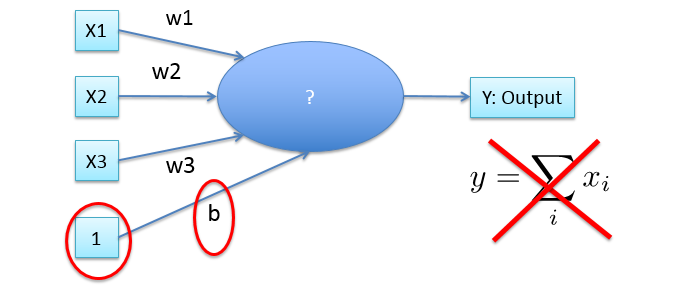
\includegraphics[width=0.8\linewidth,keepaspectratio]{ai10}
\end{center}
Does not work.
\tiny{(Reference: Neural Networks - Dr. Long Tran-Thanh)}
\end{frame}
%%%%%%%%%%%%%%%%%%%%%%%%%%%%%%%%%%%%%%%%%%%%%%%%%%%
\begin{frame}[fragile] \frametitle{Weighted sum of the inputs}
Idea 2: If we allow the possibility of weighting each input differently, we gain some expressivity 
\begin{center}
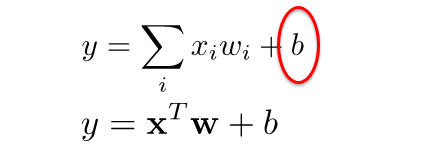
\includegraphics[width=0.6\linewidth,keepaspectratio]{ai11}
\end{center}
Remind you of anything?
\tiny{(Reference: Neural Networks - Dr. Long Tran-Thanh)}
\end{frame}

%%%%%%%%%%%%%%%%%%%%%%%%%%%%%%%%%%%%%%%%%%%%%%%%%%%
\begin{frame}[fragile] \frametitle{Weighted sum of the inputs and function}
Idea 3: Transform weighted sum via a function 
\begin{center}
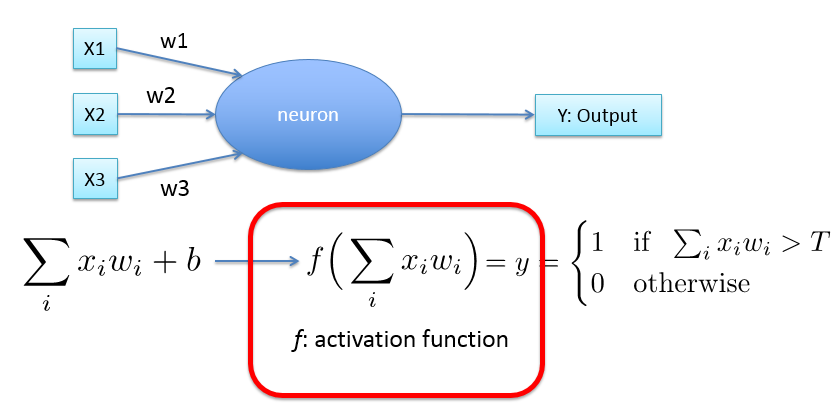
\includegraphics[width=\linewidth,keepaspectratio]{ai12}
\end{center}

\tiny{(Reference: Neural Networks - Dr. Long Tran-Thanh)}
\end{frame}

%%%%%%%%%%%%%%%%%%%%%%%%%%%%%%%%%%%%%%%%%%%%%%%%%%%
\begin{frame}[fragile] \frametitle{Transformation functions}
Activation functions
\begin{center}
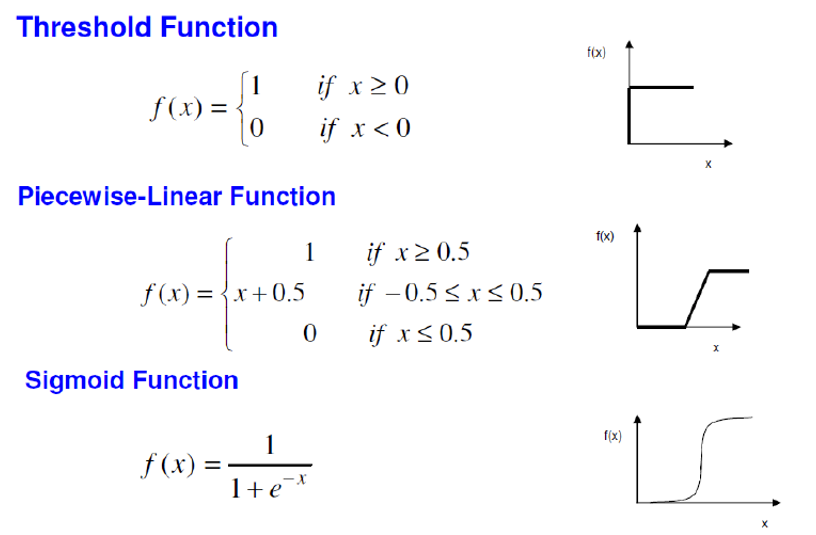
\includegraphics[width=\linewidth,keepaspectratio]{ai13}
\end{center}
\tiny{(Reference: Neural Networks - Dr. Long Tran-Thanh)}
\end{frame}

%%%%%%%%%%%%%%%%%%%%%%%%%%%%%%%%%%%%%%%%%%%%%%%%%%%%%%%%%%
\begin{frame}[fragile] \frametitle{The Training Process}
Learns by generating an error signal that measures the difference between the
predictions of the network and the desired values and then using this error signal
to change the weights (or parameters) so that predictions get more accurate.
\begin{center}
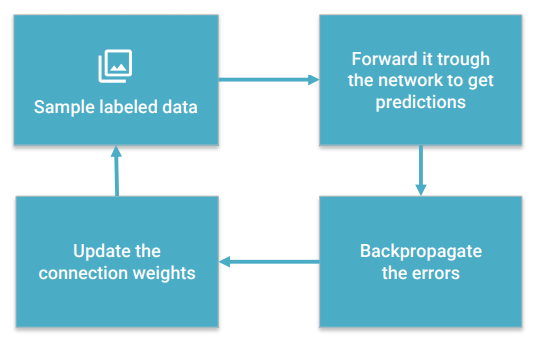
\includegraphics[width=0.6\linewidth,keepaspectratio]{ai44}
\end{center}
{\tiny (Deep Learning - The Past, Present and Future of Artificial Intelligence - Lukas Masuch)}
\end{frame}

%%%%%%%%%%%%%%%%%%%%%%%%%%%%%%%%%%%%%%%%%%%%%%%%%%%%%%%%%%
\begin{frame}[fragile] \frametitle{Gradient Descent}
Gradient Descent finds the (local) the minimum of the cost function (used to
calculate the output error) and is used to adjust the weights.
\begin{center}
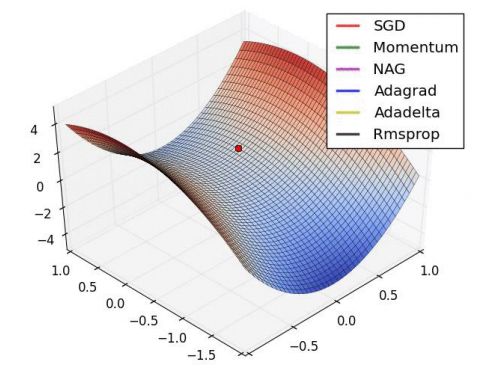
\includegraphics[width=0.6\linewidth,keepaspectratio]{ai45}
\end{center}
{\tiny (Deep Learning - The Past, Present and Future of Artificial Intelligence - Lukas Masuch)}
\end{frame}


%%%%%%%%%%%%%%%%%%%%%%%%%%%%%%%%%%%%%%%%%%%%%%%%%%%
\begin{frame}[fragile] \frametitle{Example}
Gates
\begin{center}
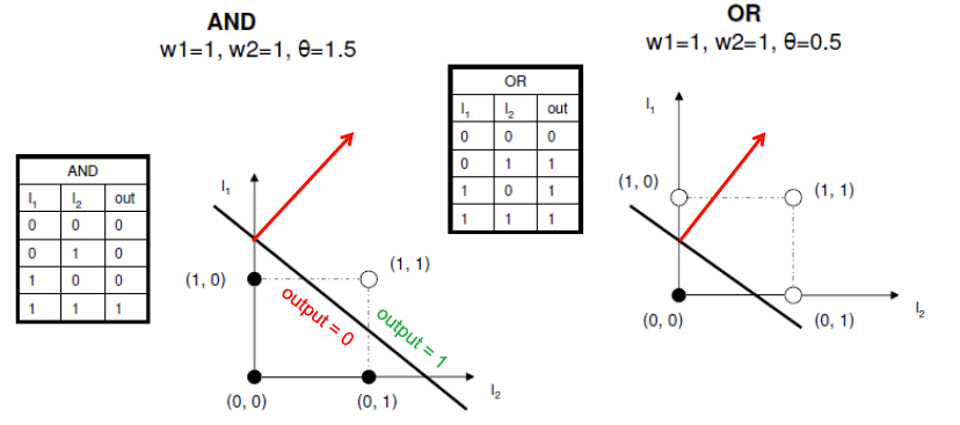
\includegraphics[width=\linewidth,keepaspectratio]{ai14}
\end{center}
\tiny{(Reference: Neural Networks - Dr. Long Tran-Thanh)}

\end{frame}

%%%%%%%%%%%%%%%%%%%%%%%%%%%%%%%%%%%%%%%%%%%%%%%%%%%
\begin{frame}[fragile] \frametitle{Example}
Gates
\begin{center}
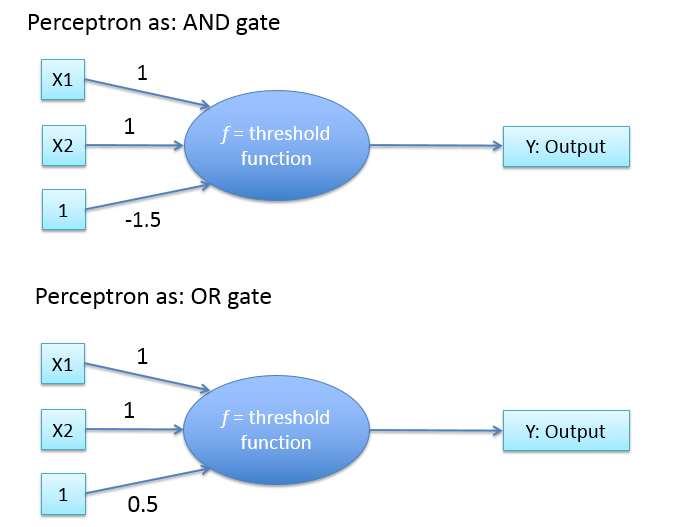
\includegraphics[width=0.7\linewidth,keepaspectratio]{ai15}
\end{center}
\tiny{(Reference: Neural Networks - Dr. Long Tran-Thanh)}

\end{frame}

%%%%%%%%%%%%%%%%%%%%%%%%%%%%%%%%%%%%%%%%%%%%%%%%%%%
\begin{frame}[fragile] \frametitle{Example}
Limitation
\begin{center}
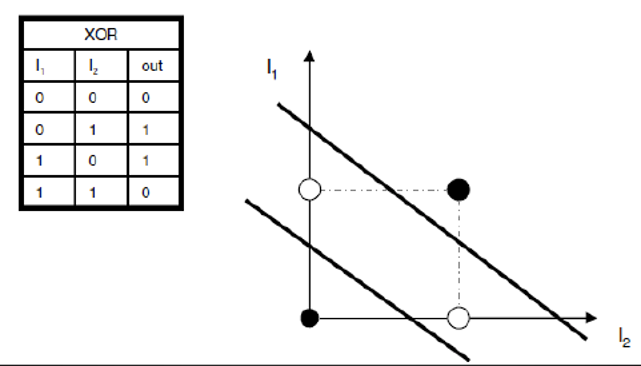
\includegraphics[width=0.7\linewidth,keepaspectratio]{ai16}
\end{center}
\tiny{(Reference: XOR gate (Minsky and Papert, 1969)}

\end{frame}

%%%%%%%%%%%%%%%%%%%%%%%%%%%%%%%%%%%%%%%%%%%%%%%%%%%
\begin{frame}[fragile] \frametitle{How to overcome?}

\begin{itemize}
\item How can we overcome this issue?
\item Possible solution: multi-layer neural nets
\item Intuition: If we think of perceptrons as dividing a space into low vs high output with a single line
\item then multiple perceptrons = multiple dividing lines
\item Non-linear separation can be approximated by a set of linear lines

\end{itemize}

\end{frame}
%%%%%%%%%%%%%%%%%%%%%%%%%%%%%%%%%%%%%%%%%%%%%%%%%%%%
%\begin{frame}[fragile] \frametitle{Human Brain}
%
%\begin{itemize}
%\item Neurons: nerve cells
%\item Neurons linked (connected) to other neurons via axons
%\item A neuron is connected to the axons via dendrites
%\item Dentrites gather inputs from other neurons
%\item  Neurons uses dendrites to gather inputs from other neurons
%\item Combines input information, and outputs a response, ``fires'' when some threshold is reached. The {\bf ``Perceptron''}.
%\item Human brain learns by changing the strength of the connection between neurons, upon repeated stimulation by the same impulse
%
%\end{itemize}
%
%\end{frame}

%%%%%%%%%%%%%%%%%%%%%%%%%%%%%%%%%%%%%%%%%%%%%%%%%%%
\begin{frame}[fragile] \frametitle{Why Deep?}

\begin{itemize}
\item Many representation multi level graph architecture. Can not be done with shallow ones like SVM, NB, etc.
\item Human Brain learns languages, speech, images, by sequence of areas
\item Humans organize their ideas and concepts hierarchically.
\item Humans first learn simpler concepts and then compose them to represent more abstract ones.
\item Engineers break-up solutions into multiple levels of abstraction and processing 
\end{itemize}
\end{frame}

%%%%%%%%%%%%%%%%%%%%%%%%%%%%%%%%%%%%%%%%%%%%%%%%%%%
\begin{frame}[fragile] \frametitle{Example}


\begin{center}
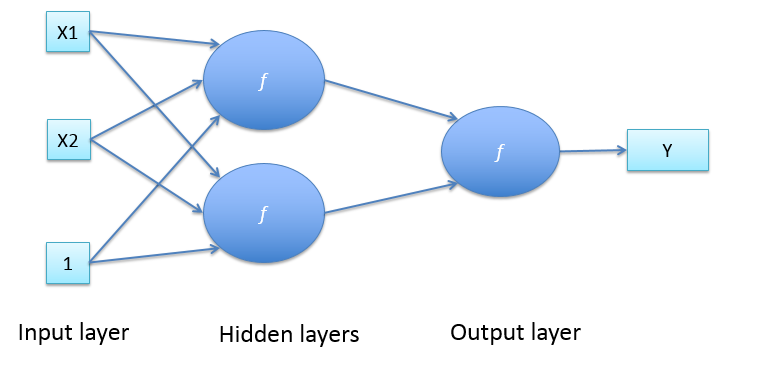
\includegraphics[width=\linewidth,keepaspectratio]{ai17}
\end{center}

Our black box is quite complicated now; can approximate arbitrary functions given enough hidden neurons. 

\tiny{(Reference: Neural Networks - Dr. Long Tran-Thanh)}

\end{frame}

%%%%%%%%%%%%%%%%%%%%%%%%%%%%%%%%%%%%%%%%%%%%%%%%%%%%%%%%%%
\begin{frame}[fragile] \frametitle{DL Network Types/Usages}
Composed of two symmetrical deep-belief networks. The encoding network learns to compresses the input to a condensed vector (dimensionality reduction). The decoding network can be used to reconstruct the data.

\begin{center}
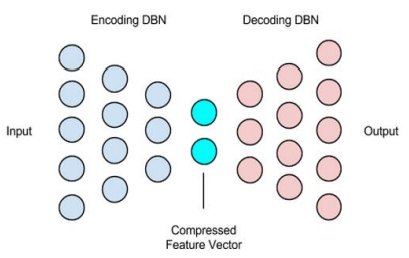
\includegraphics[width=0.4\linewidth,keepaspectratio]{ai46}
\end{center}
{\tiny (Deep Learning - The Past, Present and Future of Artificial Intelligence - Lukas Masuch)}
\end{frame}

%%%%%%%%%%%%%%%%%%%%%%%%%%%%%%%%%%%%%%%%%%%%%%%%%%%%%%%%%%
\begin{frame}[fragile] \frametitle{DL Network Types/Usages}
Convolution Neural Networks learn a complex representation of visual data
using vast amounts of data. They are inspired by the human visual system and
learn multiple layers of transformations, which are applied on top of each other to
extract a progressively more sophisticated representation of the input
\begin{center}
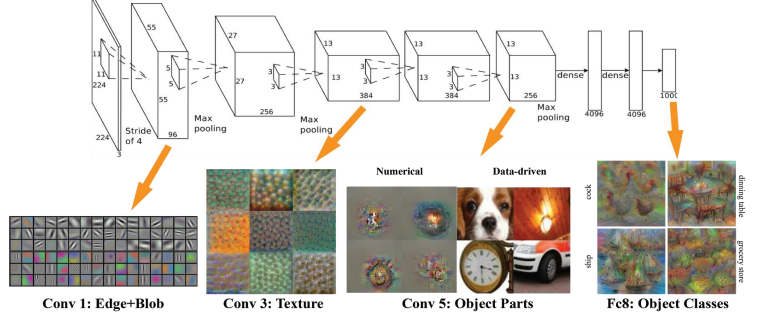
\includegraphics[width=0.6\linewidth,keepaspectratio]{ai47}
\end{center}
{\tiny (Deep Learning - The Past, Present and Future of Artificial Intelligence - Lukas Masuch)}
\end{frame}

%%%%%%%%%%%%%%%%%%%%%%%%%%%%%%%%%%%%%%%%%%%%%%%%%%%%%%%%%%
\begin{frame}[fragile] \frametitle{DL Network Types/Usages}
RNNs are general computers which can learn algorithms to map input
sequences to output sequences (flexible-sized vectors). The output
vector’s contents are influenced by the entire history of inputs. 
\begin{center}
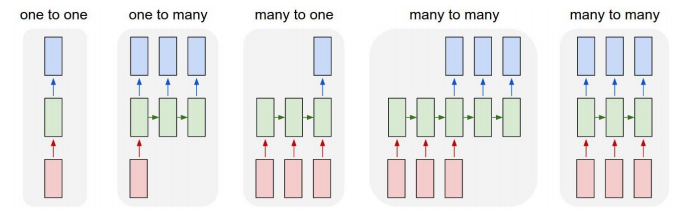
\includegraphics[width=0.6\linewidth,keepaspectratio]{ai48}
\end{center}
{\tiny (Deep Learning - The Past, Present and Future of Artificial Intelligence - Lukas Masuch)}
\end{frame}

%%%%%%%%%%%%%%%%%%%%%%%%%%%%%%%%%%%%%%%%%%%%%%%%%%%%%%%%%%
\begin{frame}[fragile] \frametitle{DL Network Types/Usages}
Generative Adversarial Networks (GANs) consist of any two networks with one tasked
to generate content and the other has to judge content. The discriminating network
receives either training data or generated content from the generative network and
tries to predict the data source (real or fake). This creates a form of competition
where the discriminator is getting better at distinguishing real data from generated
data and the generator is learning to become less predictable to the discriminator. 

\begin{center}
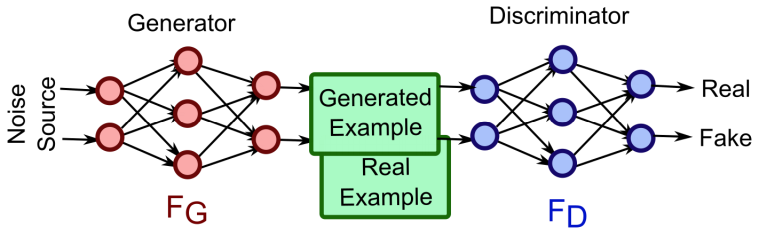
\includegraphics[width=0.6\linewidth,keepaspectratio]{ai49}
\end{center}
{\tiny (Deep Learning - The Past, Present and Future of Artificial Intelligence - Lukas Masuch)}
\end{frame}


%%%%%%%%%%%%%%%%%%%%%%%%%%%%%%%%%%%%%%%%%%%%%%%%%%%%%%%%%%
\begin{frame}[fragile] \frametitle{DL Network Types/Usages}
Natural Language Processing - Word2Vec. Vector representations of words.

\begin{center}
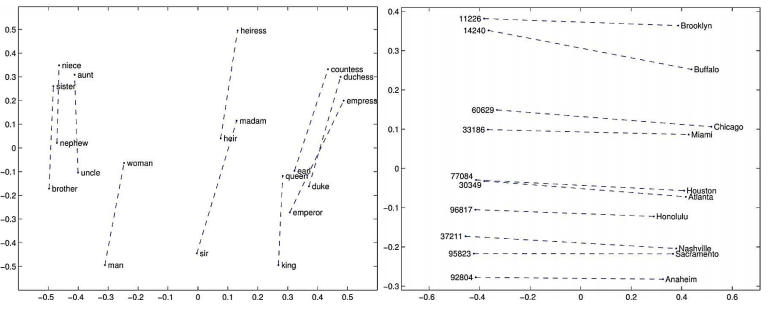
\includegraphics[width=\linewidth,keepaspectratio]{ai50}
\end{center}
{\tiny (Deep Learning - The Past, Present and Future of Artificial Intelligence - Lukas Masuch)}
\end{frame}

%%%%%%%%%%%%%%%%%%%%%%%%%%%%%%%%%%%%%%%%%%%%%%%%%%%%%%%%%%%%%%%%%%%%%%%%%%%%%%%%%%
\begin{frame}[fragile]\frametitle{Usage Requirements}
\begin{itemize}
\item Large data set with good quality (input-output mappings)
\item Measurable and describable goals (define the cost)
\item Enough computing power (AWS GPU Instance)
\item Excels in tasks where the basic unit (pixel, word) has very little
meaning in itself, but the combination of such units has a useful
meaning.
\end{itemize}
{\tiny (Deep Learning - The Past, Present and Future of Artificial Intelligence - Lukas Masuch)}
\end{frame}

%%%%%%%%%%%%%%%%%%%%%%%%%%%%%%%%%%%%%%%%%%%%%%%%%%%
\begin{frame}[fragile] \frametitle{Where do you find Deep Learning?}

\begin{itemize}
\item Speech Recognition: Siri, Alexa
\item Natural Language Processing: Google Translate
\item Image Recognition: Cancer detection
\end{itemize}
\begin{center}
\includegraphics[width=0.8\linewidth,keepaspectratio]{dl22}
\end{center}
\end{frame}

%%%%%%%%%%%%%%%%%%%%%%%%%%%%%%%%%%%%%%%%%%%%%%%%%%%%%%%%%%%%%%%%%%%%%%%%%%%%%%%%%%
\begin{frame}[fragile]\frametitle{Industry wants Intelligence}
\begin{center}
\includegraphics[width=\linewidth,keepaspectratio]{dl30}
\end{center}
{\tiny (Deep Learning - The Past, Present and Future of Artificial Intelligence - Lukas Masuch)}
\end{frame}

%%%%%%%%%%%%%%%%%%%%%%%%%%%%%%%%%%%%%%%%%%%%%%%%%%%%%%%%%%%%%%%%%%%%%%%%%%%%%%%%%%
\begin{frame}[fragile]\frametitle{ImageNet: The ``computer vision World Cup''}
Cats and Dogs.
\begin{center}
\includegraphics[width=\linewidth,keepaspectratio]{ai38}
\end{center}
{\tiny (Deep Learning - The Past, Present and Future of Artificial Intelligence - Lukas Masuch)}
\end{frame}

%%%%%%%%%%%%%%%%%%%%%%%%%%%%%%%%%%%%%%%%%%%%%%%%%%%%%%%%%%%%%%%%%%%%%%%%%%%%%%%%%%
\begin{frame}[fragile]\frametitle{ImageNet: The ``computer vision World Cup''}
Cats and Dogs.
\begin{center}
\includegraphics[width=\linewidth,keepaspectratio]{ai39}
\end{center}
{\tiny (Deep Learning - The Past, Present and Future of Artificial Intelligence - Lukas Masuch)}
\end{frame}



%%%%%%%%%%%%%%%%%%%%%%%%%%%%%%%%%%%%%%%%%%%%%%%%%%%
\begin{frame}[fragile] \frametitle{Heroes of Deep Learning}

\begin{center}
\includegraphics[width=\linewidth,keepaspectratio]{ai18}
\end{center}

\tiny{(Reference: Neural Networks - Dr. Long Tran-Thanh)}
\end{frame}


%%%%%%%%%%%%%%%%%%%%%%%%%%%%%%%%%%%%%%%%%%%%%%%%%%%%%%%%%%%%%%%%%%%%%%%%%%%%%%%%%%
\begin{frame}[fragile]\frametitle{Big Players}
Companies
\begin{center}
\includegraphics[width=\linewidth,keepaspectratio]{ai41}
\end{center}
{\tiny (Deep Learning - The Past, Present and Future of Artificial Intelligence - Lukas Masuch)}
\end{frame}

%%%%%%%%%%%%%%%%%%%%%%%%%%%%%%%%%%%%%%%%%%%%%%%%%%%%%%%%%%%%%%%%%%%%%%%%%%%%%%%%%%
\begin{frame}[fragile]\frametitle{Big Players}
Startups
\begin{center}
\includegraphics[width=\linewidth,keepaspectratio]{ai42}
\end{center}
{\tiny (Deep Learning - The Past, Present and Future of Artificial Intelligence - Lukas Masuch)}
\end{frame}
